\lab{Introduction to Plotting: Matplotlib and Mayavi}{Matplotlib and Mayavi}
\objective{Data visualization is a key component of scientific computing.
Python has several standard packages that work in conjunction with NumPy and SciPy to visualize data contained in arrays.
In this lab we introduce Matplotlib, the most commonly-used visualization library in Python.
We also introduce Mayavi, a module with extensive 3-D visualization capabilities.
These plotting techniques will be used in the majority of the labs in this curriculum.}
\label{lab:Matplotlib_and_Mayavi}


\section*{Line Plots} % =======================================================

The quickest way to visualize a simple 1-D array is via a \emph{line plot}.
In the following example, we create an array to visualize and plot it using the \li{matplotlib} module.\footnote{Like NumPy and SciPy, Matplotlib is \emph{not} part of the Python standard library, but is included in most Python distributions.}

\begin{lstlisting}
>>> import numpy as np
>>> from matplotlib import pyplot as plt

>>> y = np.array([n**2 for n in xrange(-5, 6)])
>>> y
array([25, 16,  9,  4,  1,  0,  1,  4,  9, 16, 25])

# Visualize the plot.
>>> plt.plot(y)                     # Draw the line plot.
<<[<matplotlib.lines.Line2D object at 0x1084762d0>]>>
>>> plt.show()                      # Reveal the resulting plot.
\end{lstlisting}

The result is shown in Figure \ref{fig:basic1}.
Just as \li{np} is a standard alias for NumPy, \li{plt} is a standard alias for \li{matplotlib.pyplot} in the Python community.

The call \li{plt.plot(y)} creates a figure and draws straight lines connecting the entries of \li{y} relative to the $y$-axis.
The $x$-axis is by default the index of the array, namely the integers from $0$ to $10$.
Calling \li{plt.show()} then displays the figure.

\begin{figure}[H] % plt.plot(y) compared to plt.plot(x,y).
\captionsetup[subfigure]{justification=centering}
\centering
\begin{subfigure}{.5\textwidth}
    \centering
    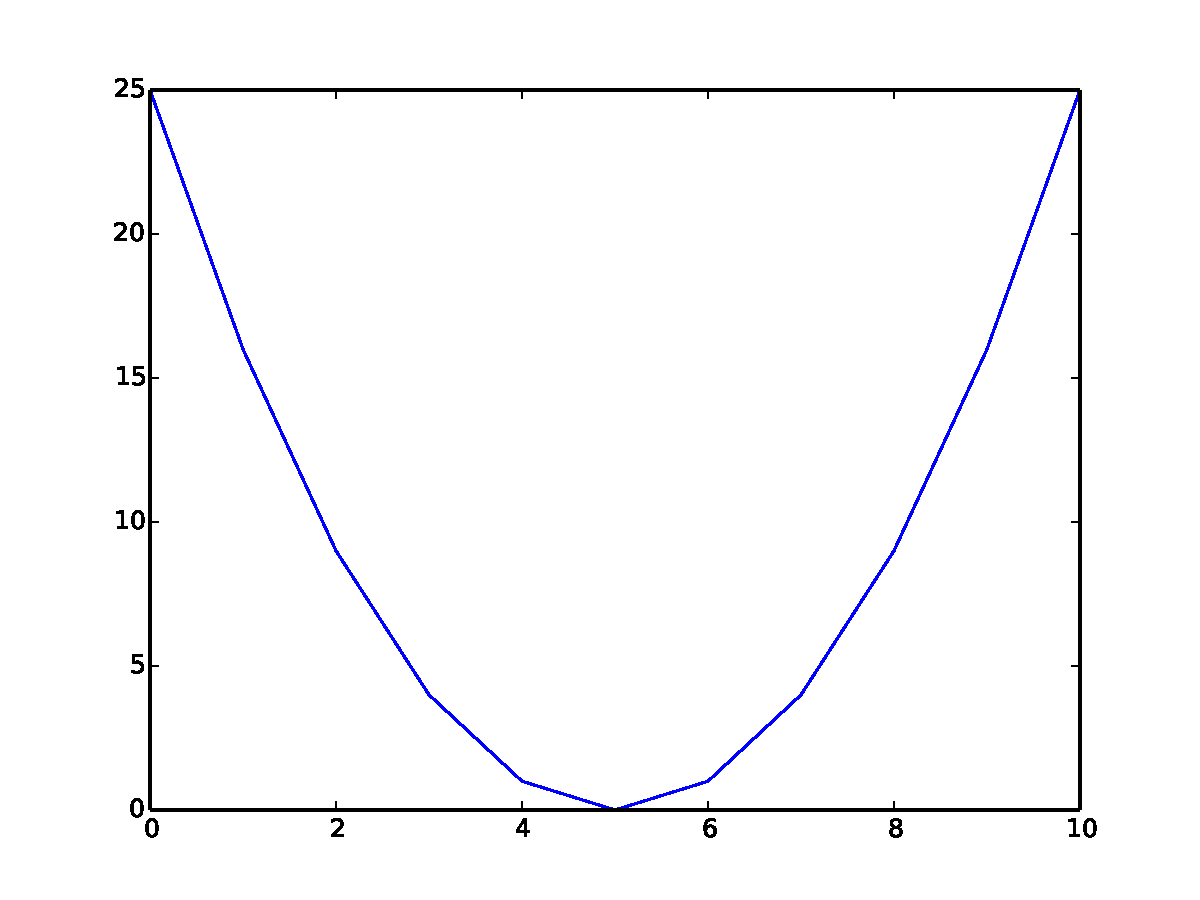
\includegraphics[width=\linewidth]{basic1.pdf}
    \caption{\li{plt.plot(y)} uses the indices of\\the array for the $x$-axis.}
    \label{fig:basic1}
\end{subfigure}%
\begin{subfigure}{.5\textwidth}
    \centering
    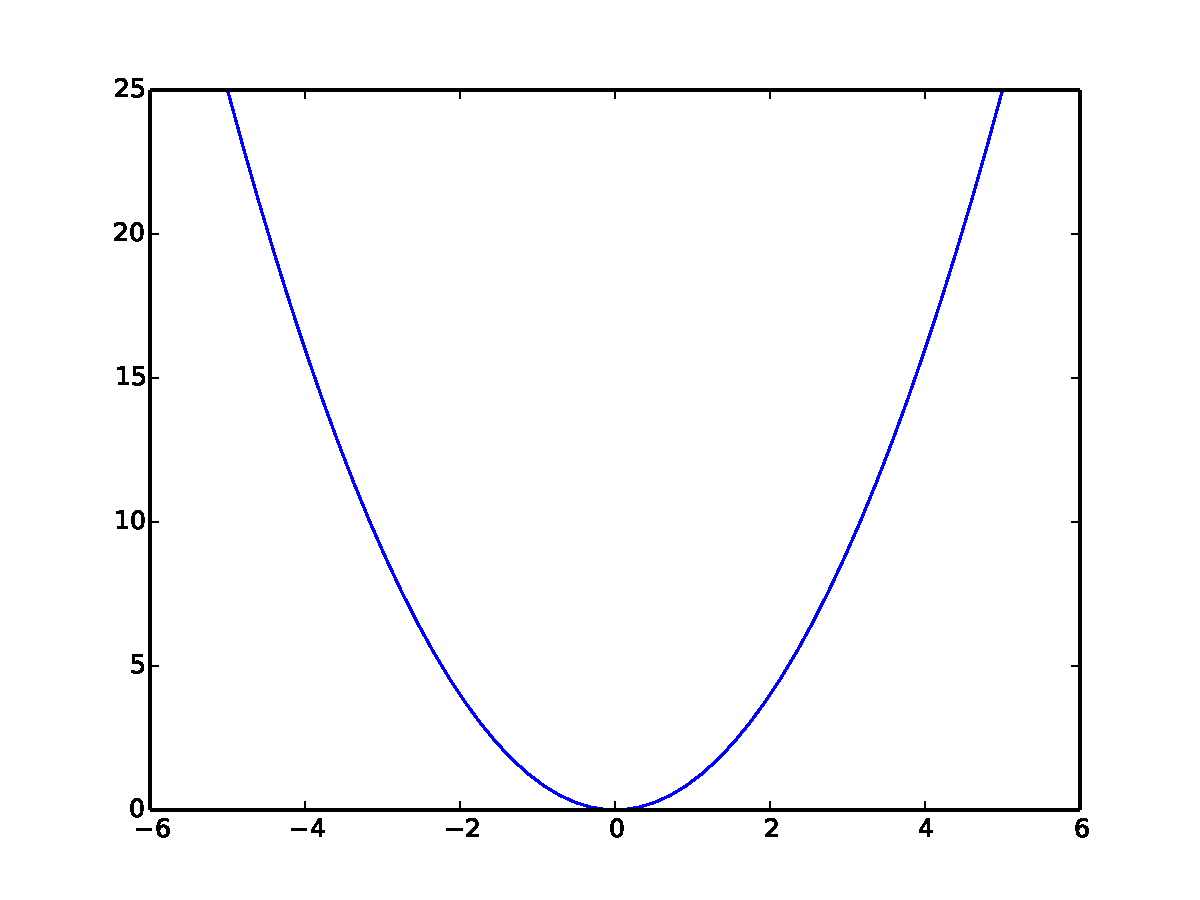
\includegraphics[width=\linewidth]{basic2.pdf}
    \caption{\li{plt.plot(x,y)} specifies both the\\domain and the range.}
    \label{fig:basic2}
\end{subfigure}
\caption{Simple plots of $f(x) = x^2$ over the interval $x\in[-5,5]$.}
\end{figure}

\begin{problem} % Law of Large Numbers / NumPy review.
Write a function that accepts an integer $n$ as input.
\begin{enumerate}
\item Use \li{np.random.randn()} or \li{np.random.normal()} to create an $n\times n$ array of values randomly sampled from the standard normal distribution.
\item Compute the mean of each row of the array.
\\(Hint: use \li{np.mean()} and specify the \li{axis} keyword argument.)
\item Return the variance of these means (this should be a single scalar).
\end{enumerate}
Define a new function that creates an array of the results of the first function with inputs $n = 100,\ 200,\ \ldots,\ 1000$.
% \begin{lstlisting}
% >>> y = np.array([prob1(n) for n in xrange(100,1100,100)])
% \end{lstlisting}
%
Plot (and show) the resulting array.

This illustrates one version of the \emph{Law of Large Numbers}, which will be discussed later on in Volume II.
\end{problem}

\subsection*{Specifying a Domain} % -----------------------------------------

An obvious problem with Figure \ref{fig:basic1} is that the $x$-axis does not correspond correctly to the $y$-axis for the function $f(x) = x^2$ that is being drawn.
To correct this, we provide an array for the domain as well as one for the range.
That is, we first define an array \li{x} for the domain, then use that array to calculate the range \li{y} of the function we would like to plot.
The command \li{plt.plot(x,y)} then plots \li{x} against \li{y}.
That is, each point \li{(x[i], y[i])} is drawn and consecutive points are connected.
% Thus both arrays must have the same number of elements to be compatible.

Another problem with Figure \ref{fig:basic1} is its poor resolution; the curve is visibly bumpy, especially near the bottom of the curve.
NumPy's \li{np.linspace()} function makes it easy to get a higher-resolution domain.
Recall that \li{range()} and \li{np.arange()} return a list or array of evenly-spaced values in a given interval, where the \emph{spacing} between the entries is specified.
In contrast, \li{np.linspace()} creates an array of evenly-spaced values in a given interval where the \emph{number of elements} is specified.

\begin{lstlisting}
# 4 evenly-spaced values between 0 and 32 (including endpoints).
>>> np.linspace(0, 32, 4) 
array([  0.        ,  10.66666667,  21.33333333,  32.        ])

# Get 50 evenly-spaced values from -5 to 5 (including endpoints).
>>> x = np.linspace(-5, 5, 50)
>>> y = x**2                        # Calculate the range of f(x) = x**2.
>>> plt.plot(x, y)
>>> plt.show()
\end{lstlisting}

The resulting plot is shown in Figure \ref{fig:basic2}.
Note that this time, the $x$-axis is correctly aligned with the $y$-axis.
The resolution is also much better because \li{x} and \li{y} have $50$ entries each instead of only $10$.

All calls to \li{plt} functions modify the same figure until \li{plt.show()} is executed, which displays the current figure and resets the system.
The next time a \li{plt} function is called a new figure is created.
This makes it possible to plot several lines in a single figure.

\begin{comment} % Wordy details and unnecessary plots for multi-line plotting.
We can take advantage of this system to plot multiple lines on the same axes.
For example, the following code plots ten lines, each with random values at integers from 1 to 10. 
The output is in Figure \ref{fig:statemachine}.

\begin{lstlisting}
x = np.linspace(1, 10, 10)

# Create a 10x10 array of uniformly distributed values in [0,1).
y = np.random.rand(10, 10)

# Plot each row of y
for row in y:
    plt.plot(x, row)
plt.show()
\end{lstlisting}

Alternatively, we can produce the same graph with a single call to \li{plt.plot()}.

\begin{lstlisting}
plt.plot(x, y[0], x, y[1], x, y[2], x, y[3], x, y[4], x, y[5], x, y[6], x, y[7], x, y[8], x, y[9])
plt.show()
\end{lstlisting}
\end{comment}

\begin{problem} % Plot two lines (sin() and cos()).
Plot the functions $\sin(x)$, $\cos(x)$, and $\arctan(x)$ on the domain $[-2\pi, 2\pi]$ (use \li{np.pi} for $\pi$).
% Call \li{plt.xlim(-2*np.pi, 2*np.pi)} before \li{plt.show()} to stretch the $x$-axis appropriately.
Make sure the domain is refined enough to produce a figure with good resolution.
\end{problem}

\begin{info} % Interactive Mode.
Plotting can seem a little mystical because the actual plot doesn't appear until \li{plt.show()} is executed.
Matplotlib's \emph{interactive mode}, particularly useful in IPython, allows the user to see the plot be constructed one piece at a time.
Use \li{plt.ion()} to turn interactive mode on and \li{plt.ioff()} to turn it off.
This is very useful for customizing a plot on the fly.

Try executing the following commands in IPython:

\begin{lstlisting}
In [1]: import numpy as np
In [2]: from matplotlib import pyplot as plt

# Turn interactive mode on and make some plots.
In [3]: plt.ion()
In [4]: x = np.linspace(1, 4, 100)
In [5]: plt.plot(x, np.log(x))
In [6]: plt.plot(x, np.exp(x))

# Clear the figure, then turn interactive mode off.
In [7]: plt.clf()
In [8]: plt.ioff()
\end{lstlisting}

It is wise to use interactive mode \textbf{only} with IPython, as it exhibits erratic behavior when producing subplots or multiple figures.
\end{info}

\section*{Plot Customization} % ===============================================

\li{plt.plot()} receives several keyword arguments for customizing the drawing.
For example, the color and style of the line are specified by the following string arguments.

\begin{table}[H] % Color and style.
\begin{tabular}{r|l}
    Code & Color \\
    \hline
    \li{'b'} & blue\\
    \li{'g'} & green\\
    \li{'r'} & red\\
    \li{'c'} & cyan\\
    \li{'m'} & magenta\\
    % \li{'y'} & yellow\\
    \li{'k'} & black\\
    % \li{'w'} & white
\end{tabular}
\qquad
\begin{tabular}{r|l}
    Code & Style \\
    \hline
    \li{'-'}' & solid line\\
    \li{'--'} & dashed line\\
    \li{'-.'} & dash-dot line\\
    \li{':'} & dotted line\\
    % \li{'.'} & point marker\\
    \li{'o'} & circle marker\\
    % \li{'*'} & star marker\\
    \li{'+'} & plus marker
\end{tabular}
% \caption{Common colors and line styles. See Appendix \ref{mpltables} for more.}
\end{table}

Specify one or both of these string codes as an argument to \li{plt.plot()} to change from the default color and style.
Other \li{plt} functions further customize a figure.

\begin{table}[H]
\centering
\begin{tabular}{r|l}
    Function & Description\\
    \hline
    % \li{grid()} & Add grid lines\\
    \li{legend()} & Place a legend in the plot\\
    % \li{text()} & Add text at a given position on the plot\\
    \li{title()} & Add a title to the plot\\
    \li{xlim()} & Set the limits of the $x$-axis\\
    \li{ylim()} & Set the limits of the $y$-axis\\
    % \li{xticks()} & set the location of the tick marks on the x axis, returns current locations if no arguments are given\\
    % \li{yticks()} & set the location of the tick marks on the y axis, returns current locations if no arguments are given\\
    \li{xlabel()} & Add a label to the $x$-axis\\
    \li{ylabel()} & Add a label to the $y$-axis
\end{tabular}
\end{table}

\begin{lstlisting}
>>> x1 = np.linspace(-2, 4, 100)
>>> plt.plot(x1, np.exp(x1), 'g:', linewidth=2, label="Exponential")
>>> plt.title("This is the title.", fontsize=18)
>>> plt.legend(loc="upper left")    # plt.legend() uses the 'label' argument of
>>> plt.show()                      # plt.plot() to create a legend.

>>> x2 = np.linspace(1, 4, 100)
>>> plt.plot(x2, np.log(x2), 'r+', linewidth=2)
>>> plt.xlim(0, 5)                  # Set the visible limits of the x axis.
>>> plt.xlabel("The x axis")        # Give the x axis a label.
>>> plt.show()
\end{lstlisting}

\begin{figure}[H] % Figure customizations.
\captionsetup[subfigure]{justification=centering}
\centering
\begin{subfigure}{.5\textwidth}
    \centering
    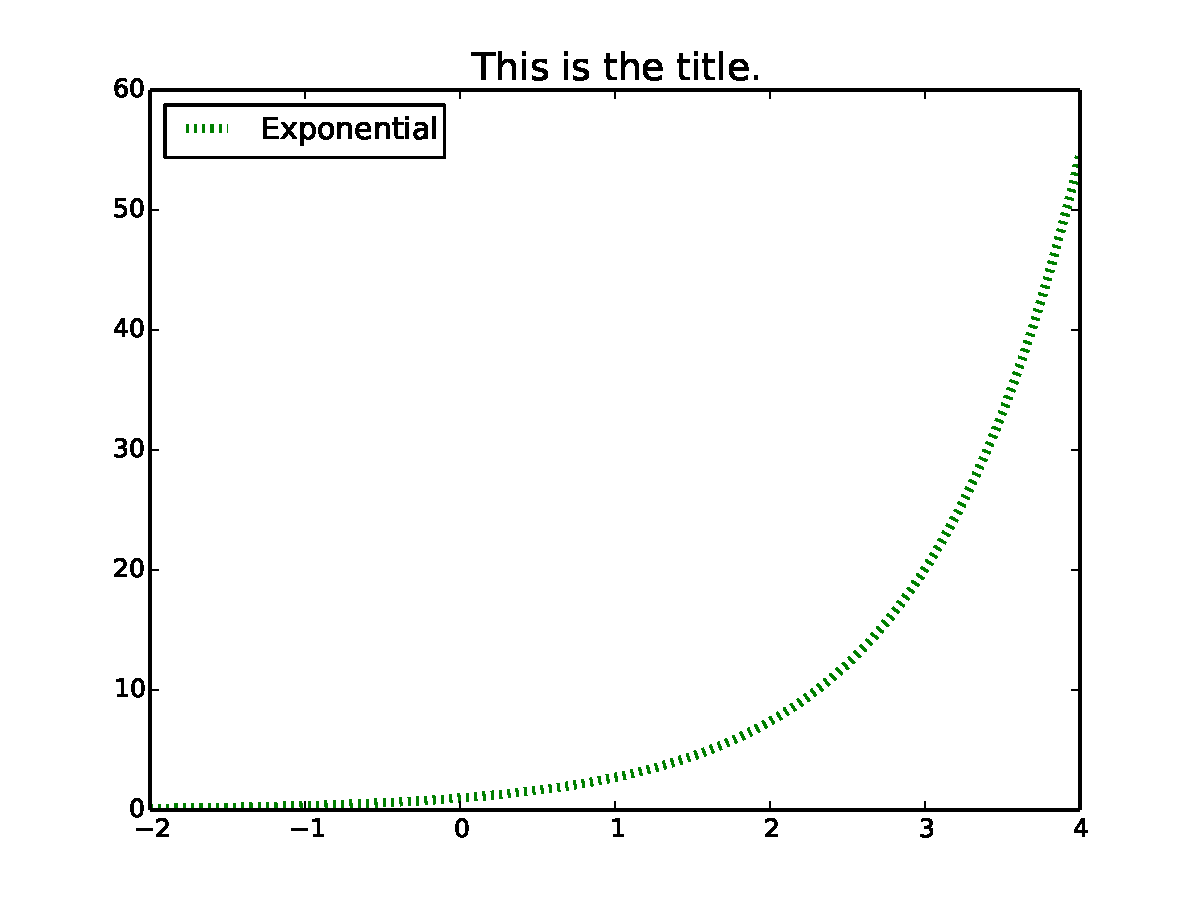
\includegraphics[width=\linewidth]{custom1.pdf}
    \label{fig:custom1}
\end{subfigure}%
\begin{subfigure}{.5\textwidth}
    \centering
    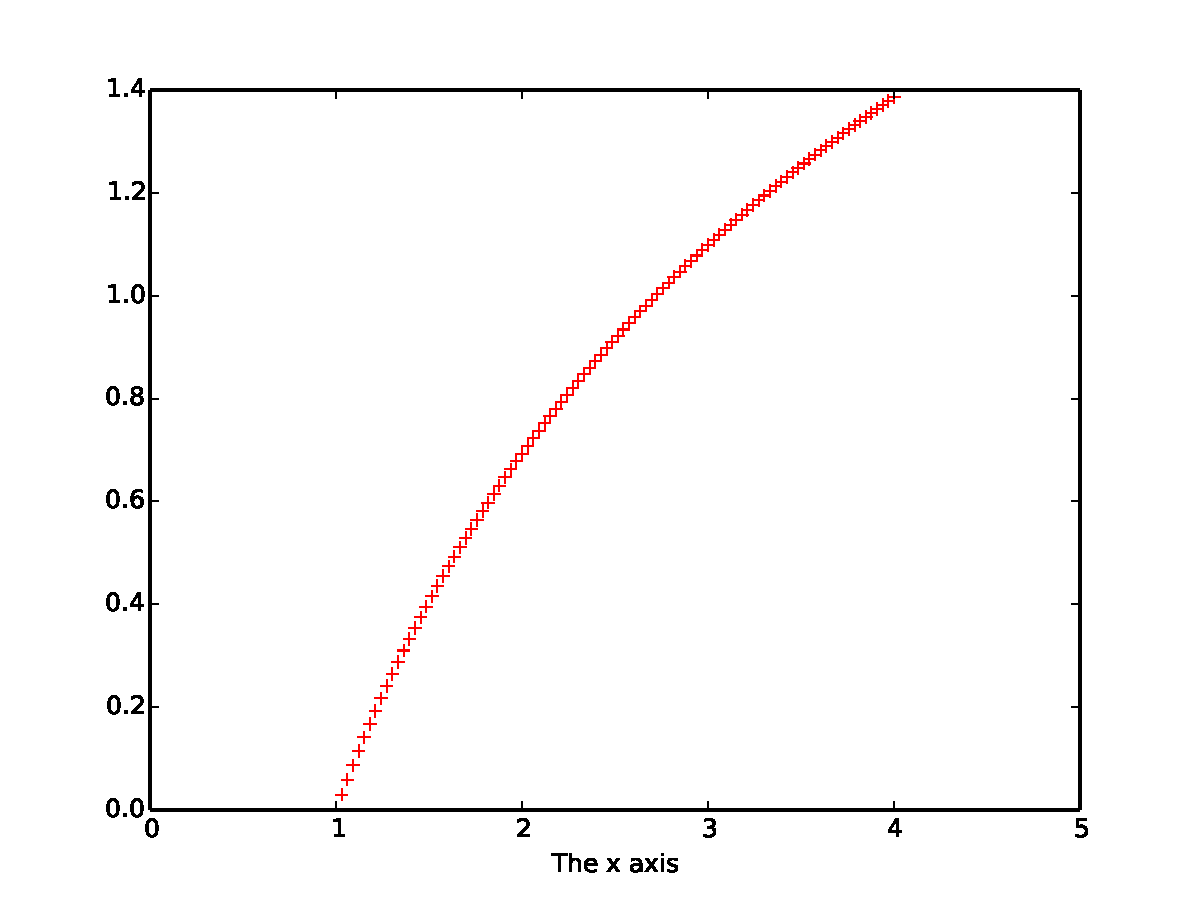
\includegraphics[width=\linewidth]{custom2.pdf}
    \label{fig:custom2}
\end{subfigure}
\label{fig:custom}
\end{figure}

See Appendix \ref{mpltables} for more comprehensive lists of colors, line styles, and figure customization routines.
    
\begin{problem} % Line plots with different domains but uniform style.
\label{prob:lineplot}
Write a function to plot the curve $f(x) = \frac{1}{x-1}$ on the domain $[-2,6]$.
Although $f(x)$ has a discontinuity at $x=1$, a single call to \li{plt.plot()} will attempt to make the curve look continuous.
\begin{enumerate}
\item Split up the domain and plot the two sides of the curve separately so that the graph looks discontinuous at $x=1$.
\item Plot both curves with a thick, dashed magenta line.\\
The keyword argument \li{linewidth} specifies the thickness of the line.
\item Change the range of the $y$-axis to be $[-6, 6]$.
\end{enumerate}
The plot should look like the figure below.

\begin{figure}[H]
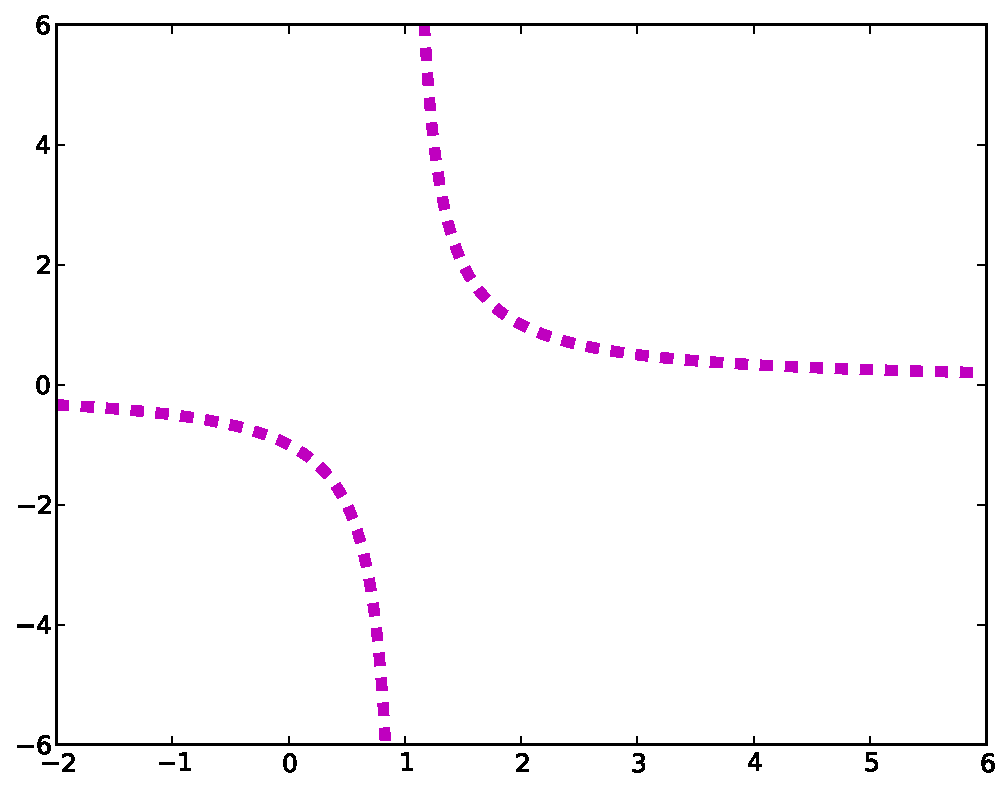
\includegraphics[width=.7\textwidth]{soln2.pdf}
\end{figure}
\end{problem}

\begin{comment} % Could still maybe be a good problem if simplified (?)
\begin{problem} Plot the curve $\frac{\sin(x)}{x+1}$ from $0$ to $10$.

Use blue shading under the curve when it is positive and red when it is negative (you may want to consider using \li{plt.fill_between()}.
Make the line dotted.
Label the x-axis ``x-axis'', the y-axis ``y-axis'',and the plot ``My Plot''.
Enable the grid lines.

Finally, use \li{plt.scatter()} to include a scatter plot of half of the value of the function at each of its maxima and minima in the range.
Display these points as upward-pointing triangles.
Don't forget to make sure the x limits of the plot are still 0 and 10.

\emph{Hint}: Since you are working with arrays of discrete values, you will want to find the index values where your $x$ and $y$ values are closest to the actual maxima and minima. As you work, consider the following:
\begin{itemize}
\item How would you manually find maxima and minima of a function?
\item How could you do something similar with your $x$ and $y$ arrays?
\end{itemize}
The plot should look like the figure below.

\begin{figure}[H]
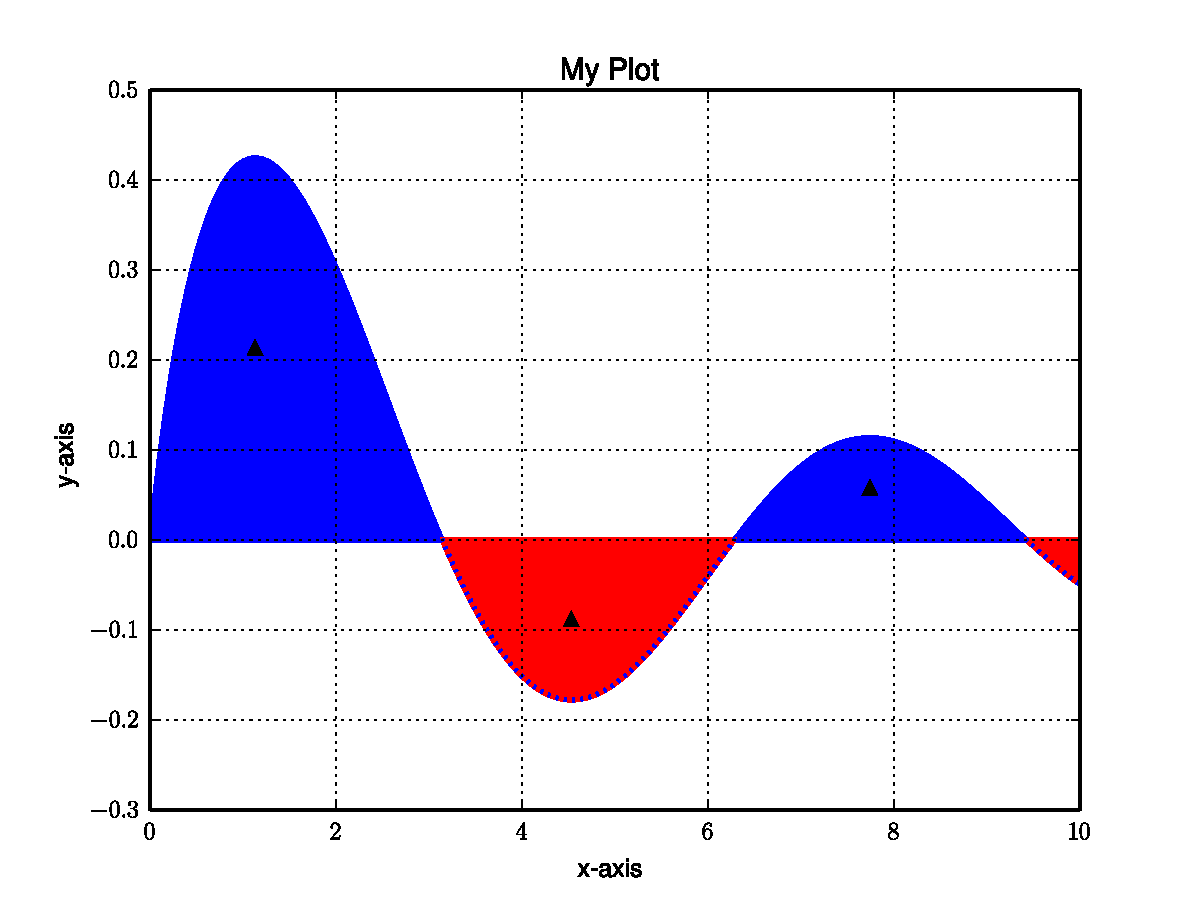
\includegraphics[width=\textwidth]{soln3.pdf}
\label{fig:problem3}
\end{figure}
\end{problem}
\end{comment}

\subsection*{Subplots} % ------------------------------------------------------

\emph{Subplots} are non-overlapping plots arranged in a grid within a single figure.
To create a figure with a grid of subplots, use \li{plt.subplot(numrows, numcols, fignum)}.
Here, \li{numrows} is the number of rows of subplots in the figure, \li{numcols} is the number of columns, and \li{fignum} specifies which subplot to modify.
% This index starts at 1 and increments across rows first.
See Figure \ref{fig:subplots}.

\begin{lstlisting}
>>> x = np.linspace(-np.pi, np.pi, 200)
>>> plt.subplot(2, 1, 1)            # Draw the first subplot.
>>> plt.plot(x, np.sin(x), 'b', linewidth=2)
>>> plt.xlim(-np.pi, np.pi)
>>> plt.subplot(2, 1, 2)            # Draw the second subplot.
>>> plt.plot(x, np.cos(x), 'c', linewidth=2)
>>> plt.xlim(-np.pi, np.pi)
>>> plt.show()                      # Show the figure with two subplots.
\end{lstlisting}

\begin{figure}[H] % Subplots
\captionsetup[subfigure]{justification=centering}
\centering
\begin{subfigure}{.49\textwidth}
    \centering
    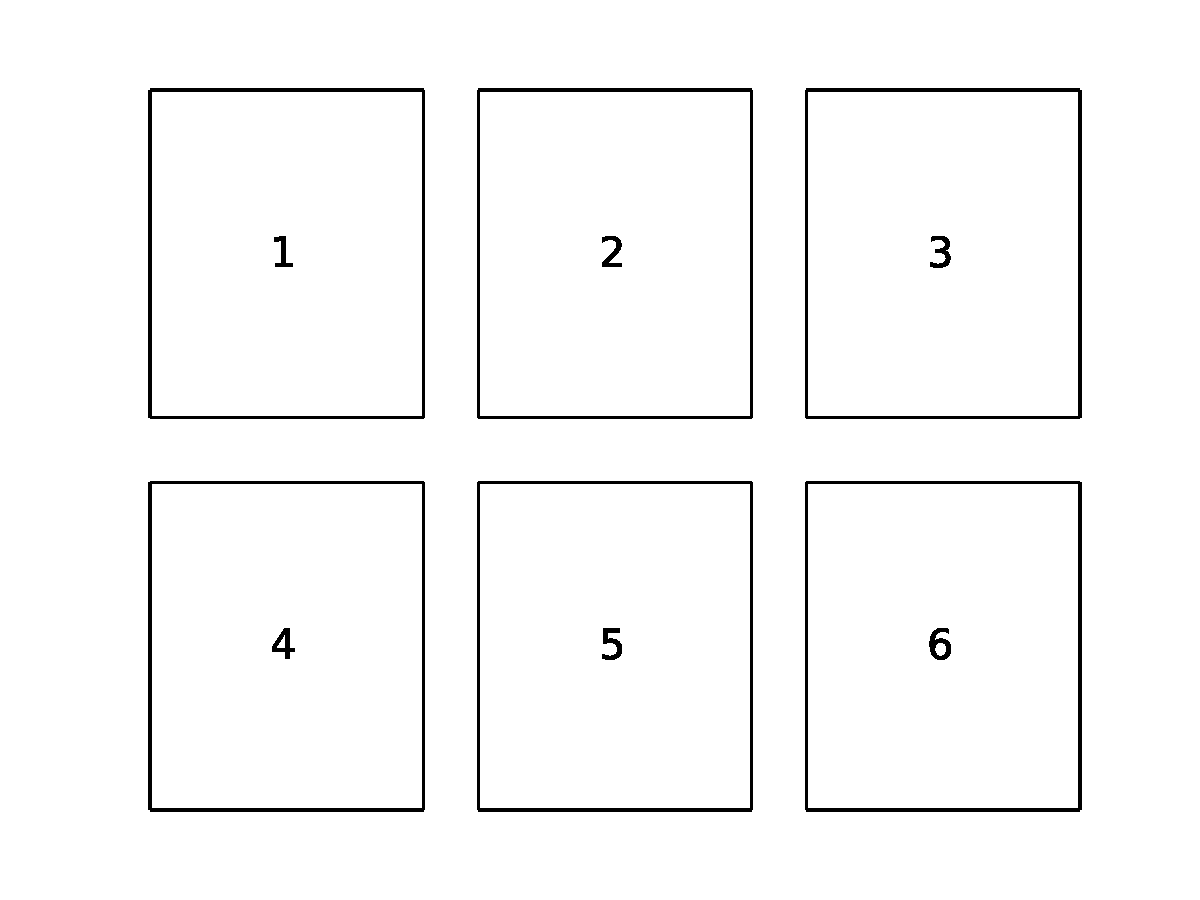
\includegraphics[width=\linewidth]{layout.pdf}
    \caption{The layout of subplots with \li{plt.subplot(2,3,i)} (2 rows, 3 columns), where \li{i} is the index pictured above.}
    \label{fig:layout}
\end{subfigure}
%
\begin{subfigure}{.49\textwidth}
    \centering
    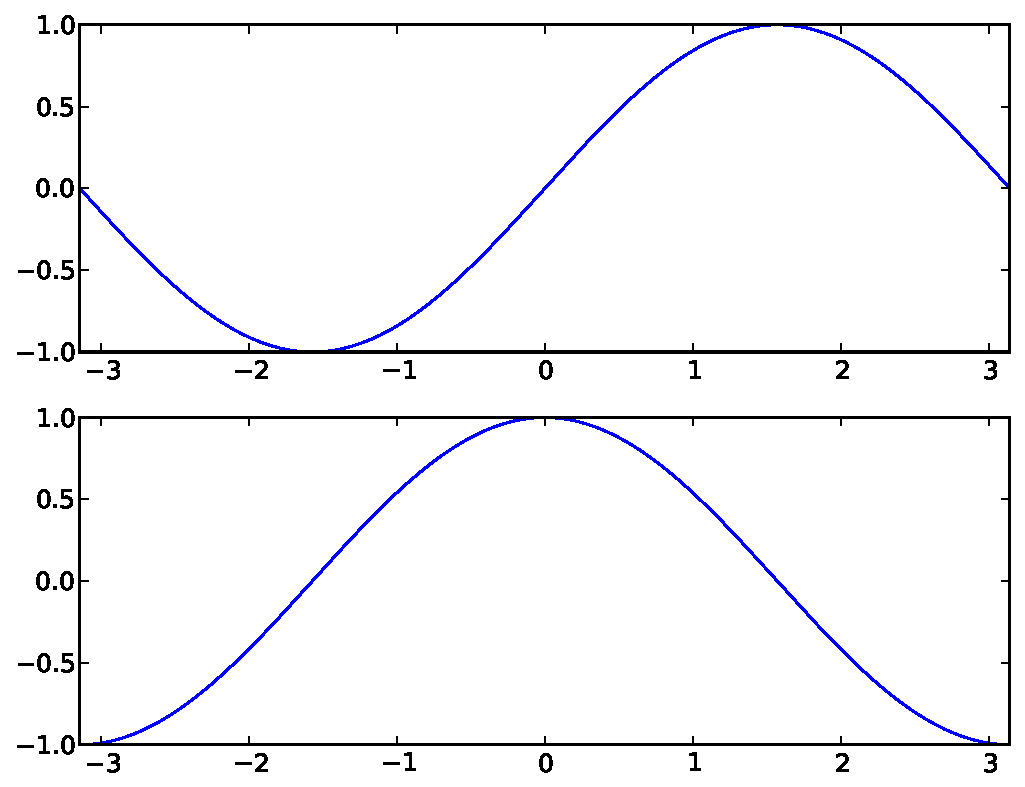
\includegraphics[width=\linewidth]{subplots.pdf}
    \caption{The graphs of $\sin(x)$ and $\cos(x)$ as subplots in a single figure with 2 rows\\and 1 column.}
    \label{fig:sincossubplots}
\end{subfigure}
\label{fig:subplots}
\end{figure}

If the inputs for \li{plt.subplot()} are all integers, the commas between the entries can be omitted.
For example, \li{plt.subplot(3,2,2)} and \li{plt.subplot(322)} are equivalent.

\begin{comment}
\begin{problem} % A new subplots problem (?)
Write a function to plot the functions $sin(x)$, $sin(2x)$, $2sin(x)$, and $2sin(2x)$ over the interval $[0, 4pi]$.
\begin{enumerate}
\item Arrange the plots in a square grid of 4 subplots.
\item Use \li{plt.title()} to give each subplot an appropriate title.
\item Use \li{plt.suptitle()} to give the overall figure a title.
\item Adjust the color and linewidth of each line to match the figure below.
\end{enumerate}
The plot should look like the figure below.

% FIGURE HERE

\end{problem}
\end{comment}

\section*{Other Kinds of Plots} % =============================================

A \emph{histogram} groups entries of a 1-D data set into a given number of intervals, called \emph{bins}.
Each bin has a bar whose height indicates the number of values that fall in the range of the bin.
To create a histogram, use \li{plt.hist()} instead of \li{plt.plot()}.
% We may specify the number of bins and the range of values to control the precision of the plot.

A \emph{scatter plot} plots two arrays against each other without drawing lines between the points.
Use \li{plt.scatter()}, or use \li{plt.plot()} and specify a point marker (such as \li{'o'} or \li{'+'}) for the line style.

\begin{lstlisting}
# Get 2 sets of 20 random integers in the interval [1, 11).
>>> x, y = np.random.randint(1, 11, 20), np.random.randint(1, 11, 20)

# Draw a histograms and a scatter plot to display the data.
>>> plt.subplot(121)
>>> plt.hist(x, bins=10, <<range>>=[.5, 10.5])
>>> plt.subplot(122)
>>> plt.scatter(x, y, s=100)        # The 's' argument specifies the marker size.
>>> plt.show()
\end{lstlisting}

\begin{figure}[H]
\centering
\begin{subfigure}{.5\textwidth}
    \centering
    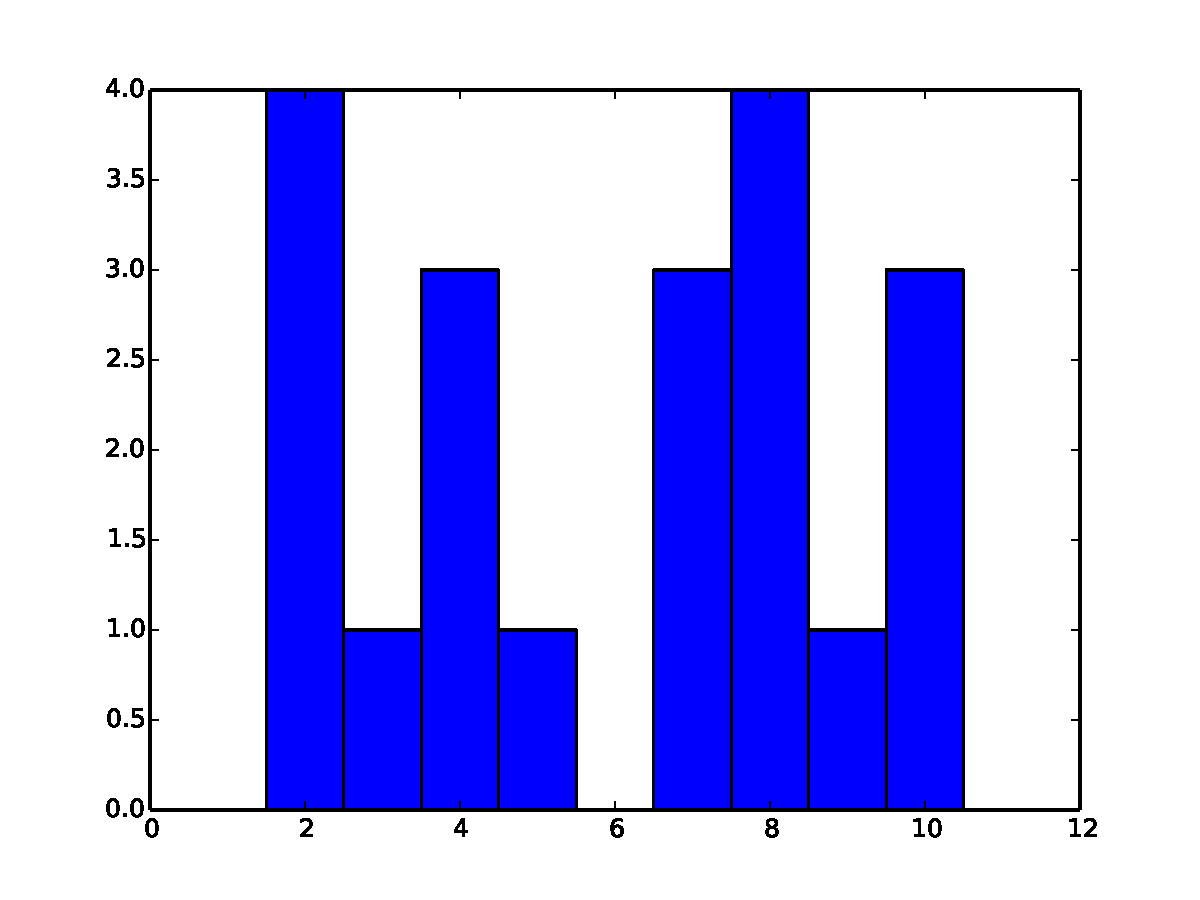
\includegraphics[width=\linewidth]{histogram.pdf}
    % \caption{A histogram.}
    \label{fig:histogram}
\end{subfigure}%
\begin{subfigure}{.5\textwidth}
    \centering
    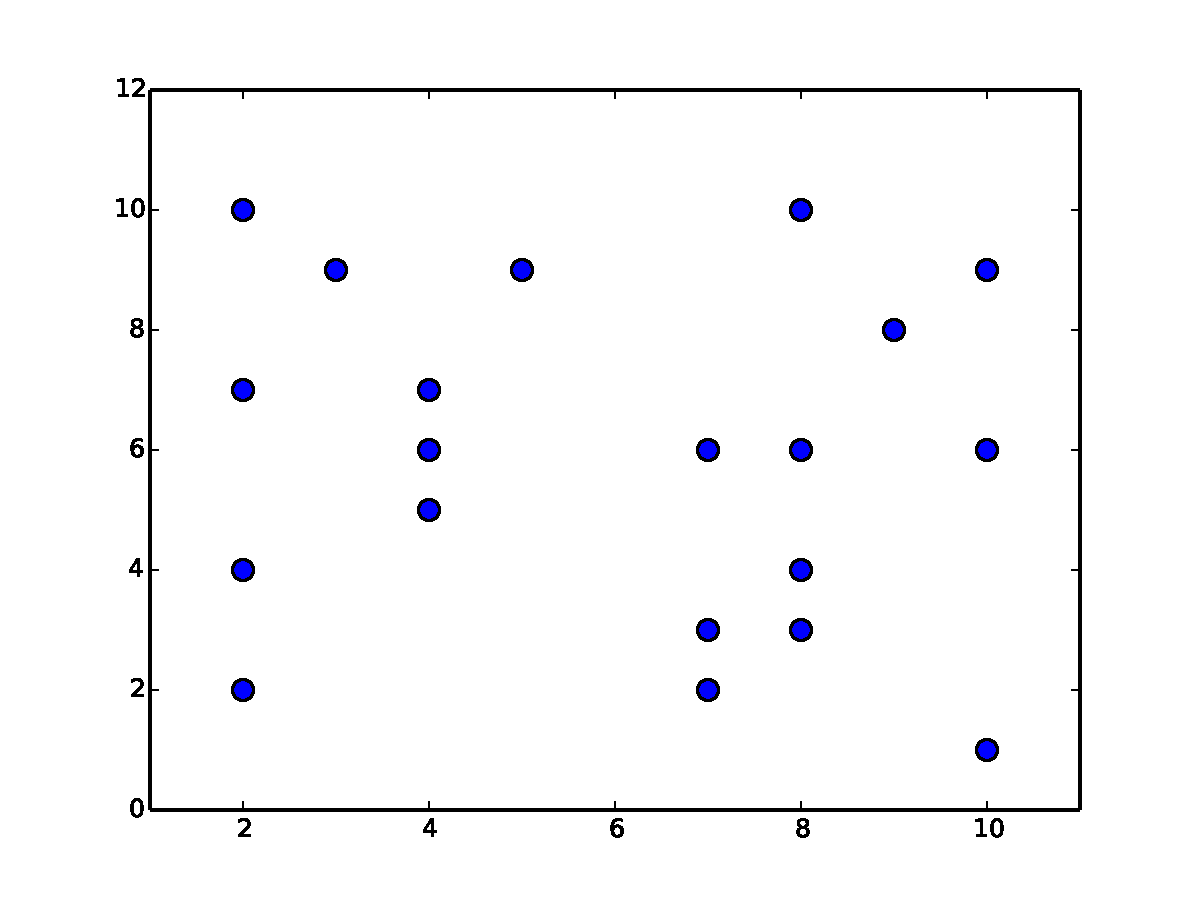
\includegraphics[width=\linewidth]{scatter.pdf}
    % \caption{A scatter plot.}
    \label{fig:scatter}
\end{subfigure}
\end{figure}

In this example the data set \li{x} consists of only integer values.
Specifying 10 bins in the range [.5, 10.5] creates one bin per integer.

\begin{problem} % Find some real data to use with this problem. age v height?
\label{prob:subplot}
The file \texttt{TODO.npz} contains some interesting data that is described here.
Use \li{np.load()} to load the two arrays in the file:
\begin{lstlisting}
>>> data = np.load("TODO.npz")
>>> x, y = data['TODO_1'], data['TODO_2']
\end{lstlisting}

Write a function to generate the following plot:
\begin{enumerate}
\item In one subplot, draw a histogram of the first array (\li{x}).
Choose an appropriate range and number of bins to display the data accurately.
\item In a second subplot, draw a scatter plot of \li{x} against \li{y}. 
Plot a red horizontal line whose height is equal to the mean of the \li{x} data.\\
(Hint: \li{plt.hlines()} may be useful.)
\end{enumerate}

\begin{figure}[H]
\centering
\begin{subfigure}{.5\textwidth}
    \centering
    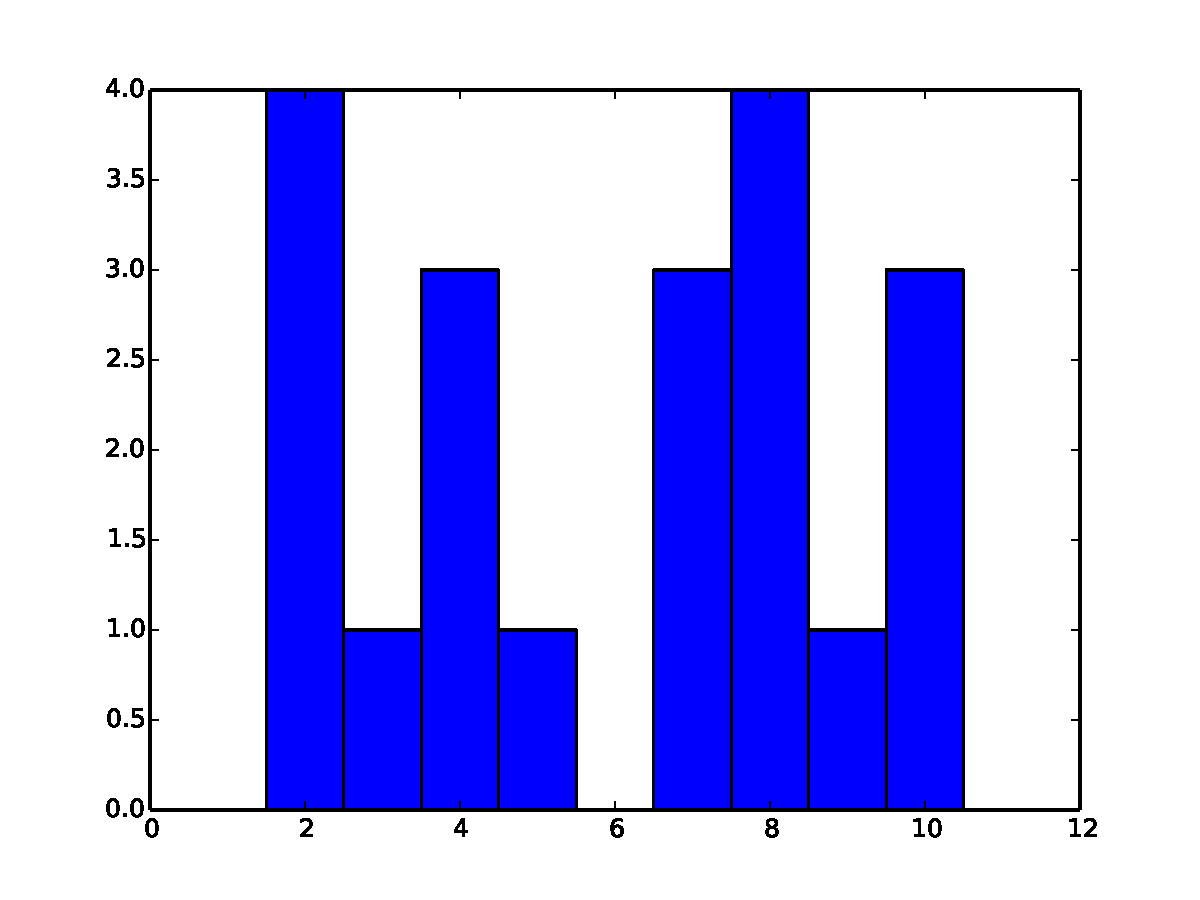
\includegraphics[width=\linewidth]{histogram.pdf}
    % \caption{A histogram.}
    \label{fig:histogram}
\end{subfigure}%
\begin{subfigure}{.5\textwidth}
    \centering
    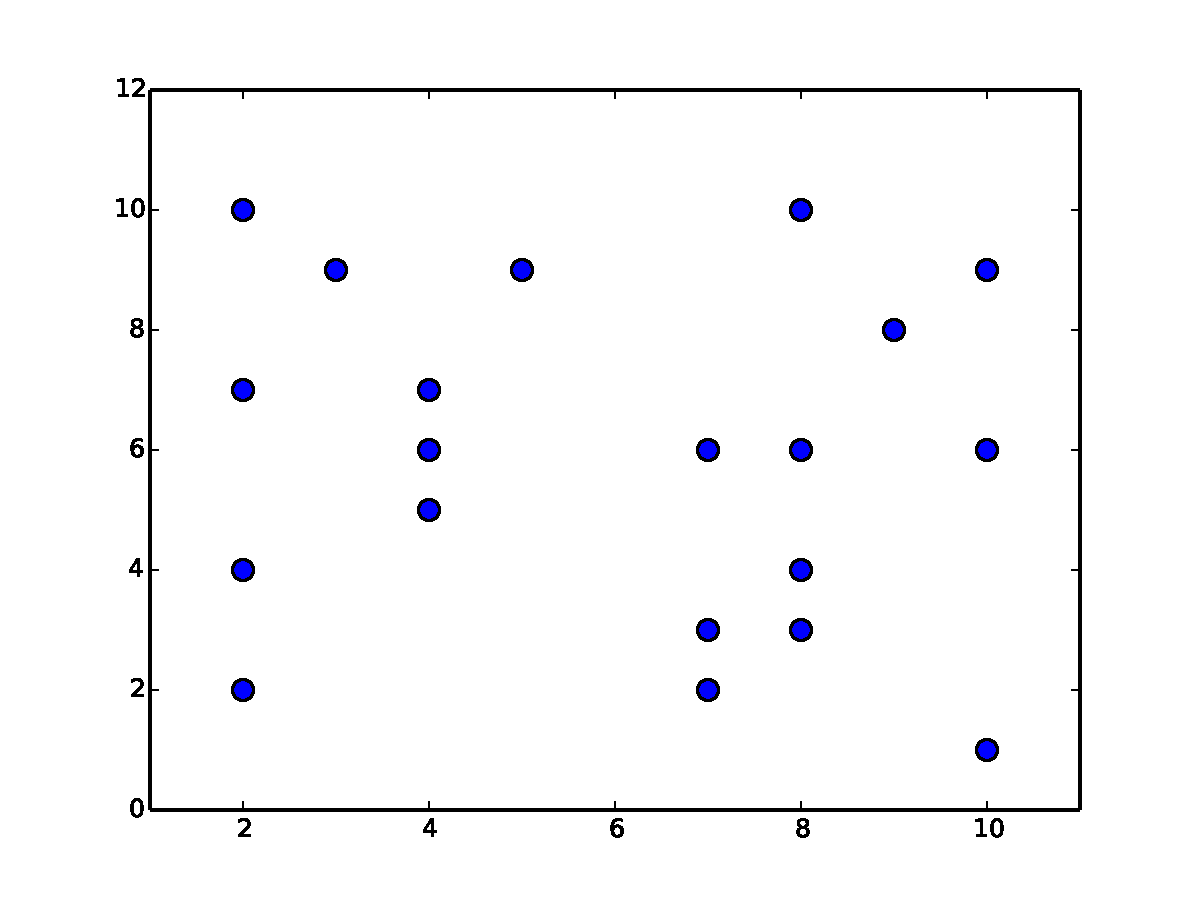
\includegraphics[width=\linewidth]{scatter.pdf}
    % \caption{A scatter plot.}
    \label{fig:scatter}
\end{subfigure}
\caption{TODO: Replace this figure (or nuke it).}
\end{figure}
\end{problem}

Other kinds of plots for 1-D data includes bar plots, box plots, and others.
See Appendix \ref{mpltables} for more.

\subsection*{Visualizing 2-D Data} % ------------------------------------------

To plot a function $f: \mathbb{R}^2 \rightarrow \mathbb{R}$, we must choose and construct a 2-D domain, then calculate the function at each point of that domain.
NumPy's \li{np.meshgrid()} is the standard tool for creating a 2-D domain in the Cartesian plane.
Given two 1-D coordinate arrays, \li{np.meshgrid()} creates two corresponding coordinate matrices.
See Figure \ref{fig:meshgrid} for a visual explanation.

\begin{figure} % np.meshgrid() visual demonstration.
\begin{tikzpicture}[>=stealth', shorten <= .1cm,shorten >=.1cm, dot/.style=
    {circle,fill=black,minimum size=3pt,inner sep=0pt, outer sep=-1pt} ]

\foreach \x/\y in {0/0, 0/2, 0/4, 2/0, 2/2, 2/4, 4/0, 4/2, 4/4} 
    \node[draw, dot]at(\x,\y){};
\foreach \x/\y in {0/0, 0/1, 0/2, 1/0, 1/1, 1/2, 2/0, 2/1, 2/2} 
    \node[draw=none]at(\x*2-.5, \y*2+.3){(\x,\y)};

\foreach \x/\y in {0/0, 0/1, 0/2, 1/0, 1/1, 1/2, 2/0, 2/1, 2/2} 
    \node[draw=none]at(\x*.75+7, \y*.75+.1){\y};
\foreach \x/\y in {0/0, 0/1, 0/2, 1/0, 1/1, 1/2, 2/0, 2/1, 2/2} 
    \node[draw=none]at(\x*.75+7, \y*-.75+3.9){\x};

\draw[-, thick](6.7,-.25)--(6.7,1.95); 
\draw[-, thick](8.8,-.25)--(8.8,1.95);
\draw[-, thick](6.7,2.05)--(6.7,4.25);
\draw[-, thick](8.8,2.05)--(8.8,4.25);
\draw[-, thick](8.8,4.14)--(8.7,4.14);
\draw[-, thick](8.8,2.16)--(8.7,2.16);
\draw[-, thick](6.7,4.14)--(6.8,4.14);
\draw[-, thick](6.7,2.16)--(6.8,2.16);
\draw[-, thick](8.8,1.84)--(8.7,1.84);
\draw[-, thick](8.8,-.135)--(8.7,-.135);
\draw[-, thick](6.8,1.84)--(6.7,1.84);
\draw[-, thick](6.8,-.135)--(6.7,-.135);

\node[draw=none](X)at(6.3,.9){\texttt{Y}=};
\node[draw=none](y)at(6.3,3.15){\texttt{X}=};

\node[draw=none](point1)at(-.3, -.6){\texttt{x}=\big[0,};
\node[draw=none, node distance=2.35cm](point2)
    [right of=point1]{1,};
\node[draw=none, node distance=2cm](point3)
    [right of=point2]{2\big]};
\node[draw=none, rotate=270](point4)at(4.6,4.25)
    {\texttt{y}=\big[2,};
\node[draw=none, rotate=270, node distance=2.35cm](point5)
    [right of=point4]{1,};
\node[draw=none, rotate=270, node distance=2cm](point6)
    [right of=point5]{0\big]};
\end{tikzpicture}
\caption{\li{np.meshgrid(x, y)}, returns the arrays \li{X} and \li{Y}. 
The returned arrays give the $x$- and $y$-coordinates of the points in the grid formed by \li{x} and \li{y}.
Specifically, the arrays \li{X} and \li{Y} satisfy \li{(X[i,j], Y[i,j]) = (x[i],y[j])}.}
\label{fig:meshgrid}
\end{figure}

With a domain, we can visualize $f$ with a \emph{heat map}.% or a \emph{surface plot}.
A heat map assigns a color to each entry in the matrix, producing a 2-D picture describing a 3-D shape.
Use \li{plt.pcolormesh()} to create a heat map.
% Matplotlib can also produce 3-D surface plots, but we will prefer to use Mayavi for 3-D plots.

\begin{lstlisting}
# Create a 2-D domain with np.meshgrid().
>>> x = np.linspace(-np.pi, np.pi, n)
>>> y = np.copy(x)
>>> X, Y = np.meshgrid(x, y)

# Calculate z = f(x,y) = sin(x)sin(y) using the meshgrid coordinates.
>>> Z = np.sin(X)*np.sin(Y)

# Plot the heat map.
>>> plt.pcolormesh(X, Y, Z)
>>> plt.colorbar()                  # Show the color scale.
>>> plt.xlim(-np.pi, np.pi)
>>> plt.ylim(-np.pi, np.pi)
>>> plt.show()
\end{lstlisting}


\begin{figure}[H] % 2D heat map vs 3D surface.
\captionsetup[subfigure]{justification=centering}
\centering
\begin{subfigure}{.5\textwidth}
    \centering
    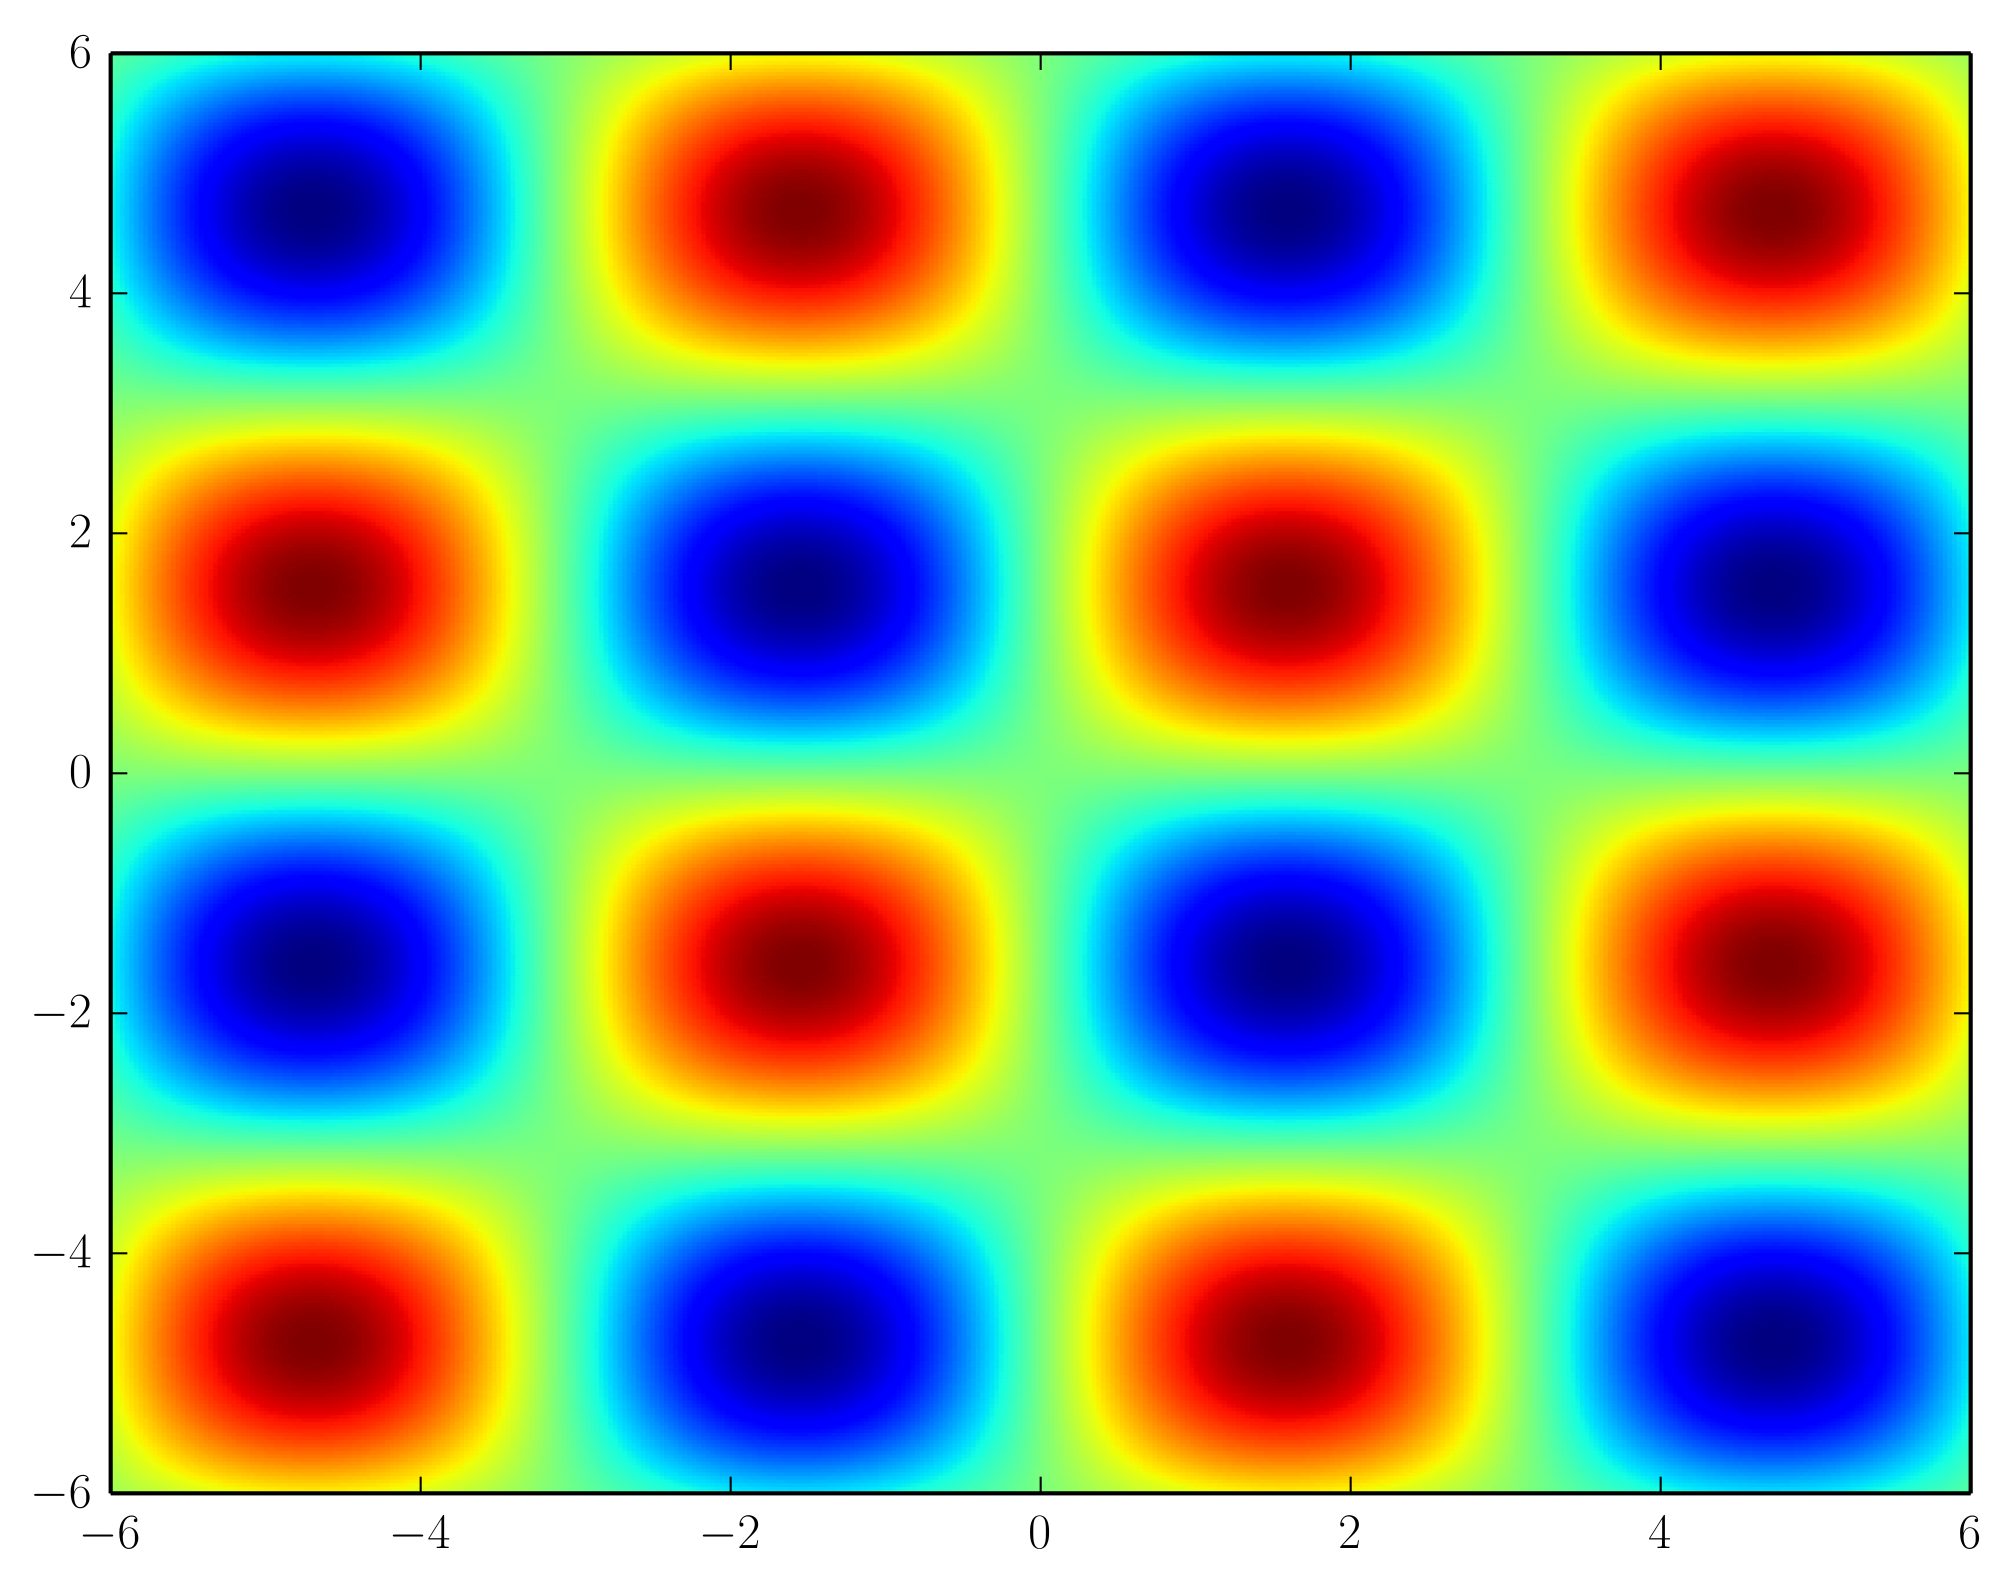
\includegraphics[width=\linewidth]{sinxsiny.png}
    \caption{A heat map of $f$.}
    \label{fig:heatmap}
\end{subfigure}%
\begin{subfigure}{.5\textwidth}
    \centering
    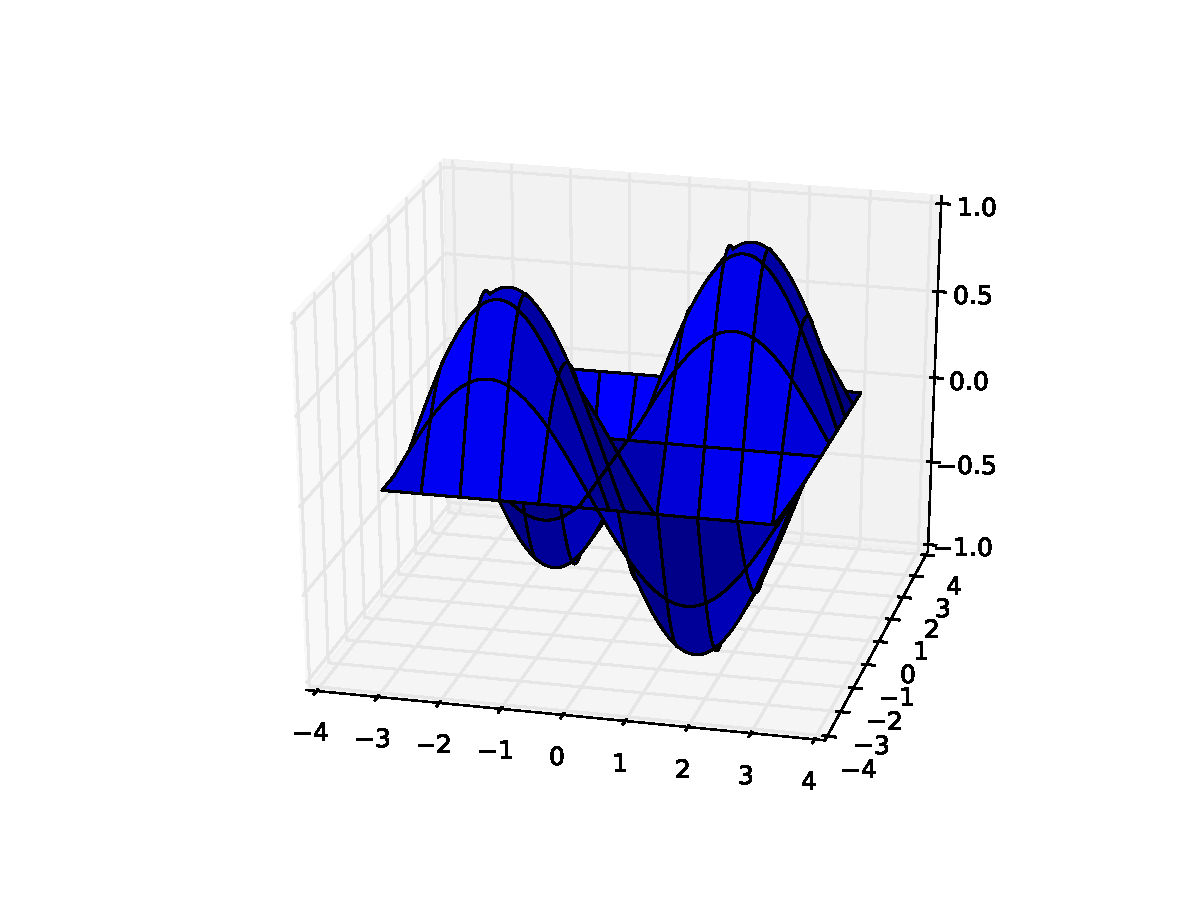
\includegraphics[width=\linewidth]{sinxsiny_3d.pdf}
    \caption{A 3-D surface plot of $f$.}
    \label{fig:surface}
\end{subfigure}
\caption{Visualization of the function $f(x,y) = \sin(x)\sin(y)$.}
\end{figure}

\begin{problem} % Heatmap problem
\label{prob:heatmap}
Write a function to plot a heat map of $f(x,y) = \frac{\sin(x)\sin(y)}{xy}$ on the domain $[-2\pi,2\pi] \times [-2\pi,2\pi]$.

\begin{enumerate}
\item The keyword \li{cmap} for \li{plt.pcolormesh()} determines the coloring scheme for the heat map.
Choose a non-default color scheme (\li{'Spectral'} is used in the figure displayed below).
For the list of all Matplotlib color schemes, see\\\url{http://matplotlib.org/examples/color/colormaps_reference.html}.
\item Include the color scale bar.
\item Change the limits on the $x$- and $y$-axes so that the plot is only over the domain $[-2\pi,2\pi] \times [-2\pi,2\pi]$.
% \item Fix the aspect ratio of your plot so that it is a square using the line \li{plt.gca().set_aspect('equal')}.
\end{enumerate}
The plot should be similar to the figure below.

\begin{figure}[H]
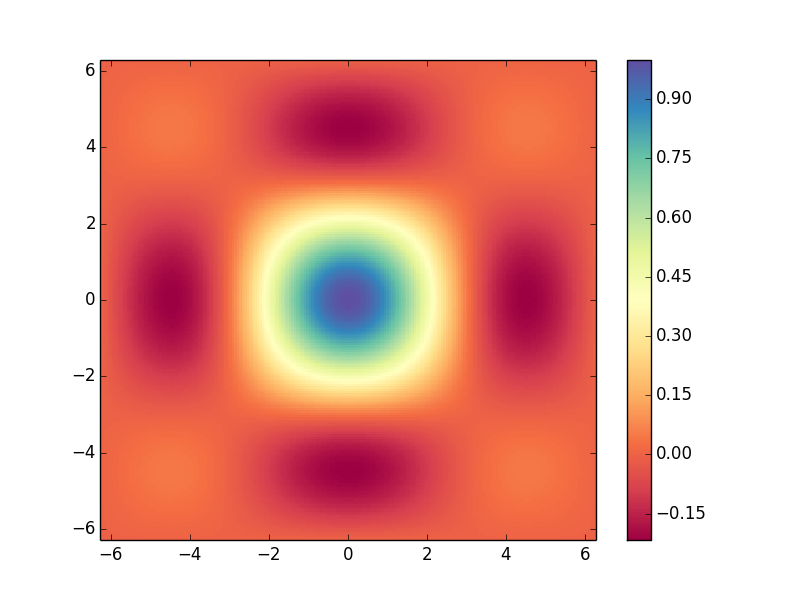
\includegraphics[width=.7\textwidth]{pcolor2.png}
% \caption{Correct output for Problem \ref{prob:heatmap}.}
% \label{fig:heatmapProb}
\end{figure}
\end{problem}

\begin{info} % Note about plt.imshow().
Images are usually stored as either a 2-D array (for black-and-white pictures) or a 3-D array (a stack of 2-D arrays, one for each RGB value).
This kind of data does not require a domain, and is easily visualized with \li{plt.imshow()}.
% We will use this function often in future labs.
\end{info}

\section*{3-D Plotting with Mayavi} % =========================================

Although Matplotlib is capable of creating 3-D plots, Mayavi\footnote{If Mayavi is not installed on your machine, run \li{conda install mayavi} from the command line. See Appendix \ref{updateinstall} for more info.} does it much faster and with better visuals.
Here we introduce methods for plotting space curves, scatter plots, and surfaces in 3-D.
The \li{mlab} submodule within the \li{mayavi} package contains the functions for creating these plots.
% We will use Mayavi for all 3-D plots in these labs. % O RLY?

\begin{warn}
Mayavi must be imported before Matplotlib.
\begin{lstlisting}
from mayavi import mlab
from matplotlib import pyplot as plt
\end{lstlisting}
\end{warn}

\begin{comment}
\begin{info} % Installation note. Make into a footnote?
If you do not have the \li{Mayavi} package installed on your system, you may download it by running the following commands from the command line:
\begin{lstlisting}
$ conda install conda               # Download the most recent installer.
$ conda install anaconda            # Update all packages.
$ conda install mayavi              # Installs mayavi.
\end{lstlisting}

% For more information regarding installing Python packages, see Appendix \ref{updateinstall}.
\end{info}

\begin{table} % Mayavi plotting functions. Probably should put this back in.
\begin{center}
\begin{tabular}
{|c|l|}
\hline
Function & Description \\
\hline
\li{barchart} & Produces 3D histogram-like plots\\
\li{contour3d} & Plots level surfaces of functions of three variables\\
\li{flow} & Creates a trajectory of particles following the flow of a vector field\\
\li{imshow} & Use a colormap to view a 2D array as an image\\
\li{mesh} & Plot a surface using \li{(x,y,z)} coordinates supplied as three 2D arrays\\
\li{plot3d} & Draws lines between points\\
\li{points3d} & Plots glyphs (like points) at the coordinates supplied\\
\li{quiver3d} & Generate 3D vector fields\\
\li{surf} & Plot a surface with a 2D array as elevation data\\
\hline
\end{tabular}
\end{center}
\caption{Some plotting functions in \li{mlab}.}
\label{table:mlab_functions}
\end{table}
\end{comment}

\subsection*{Lines} % ---------------------------------------------------------

The function \li{mlab.plot3d()} is the 3-D Mayavi equivalent for Matplotlib's \li{plt.plot()}.
Because the plot is 3-D, we must provide $x$, $y$, and $z$ coordinates, each contained in 1-D arrays of the same length.
The points \li{(x[i], y[i], z[i])} are graphed in $\mathbb{R}^3$ and connected with straight lines.

Consider the following curve, parametrized by time:
\begin{align*}
x(t) &= \cos(t)(1+\cos(6t))\\
y(t) &= \sin(t)(1+\sin(6t)\\
z(t) &= \sin\left(\frac{6}{11}t\right)
\end{align*}
The following code plots the curve over the time domain $t \in [0,2\pi]$.
The resulting plot is shown in Figure \ref{fig:plot3d}.

\begin{lstlisting}
>>> from mayavi import mlab

# Calculate the coordinates of a curve parametrized by time.
>>> t = np.linspace(0, 2*np.pi, 100)
>>> x = np.cos(t) * (1 + np.cos(t*6))
>>> y = np.sin(t) * (1 + np.cos(t*6))
>>> z = np.sin(t*6/11.)

# Plot and show the figure.
>>> mlab.plot3d(x, y, z)
>>> mlab.show()
\end{lstlisting}

\begin{figure} % Mayavi line and point plots.
\captionsetup[subfigure]{justification=centering}
\centering
\begin{subfigure}{.5\textwidth}
    \centering
    
\includegraphics[width=\linewidth]{plot3d.png}
    \caption{A 3-D curve generated by \li{mlab.plot3d()}.}
    \label{fig:plot3d}
\end{subfigure}%
\begin{subfigure}{.5\textwidth}
    \centering
    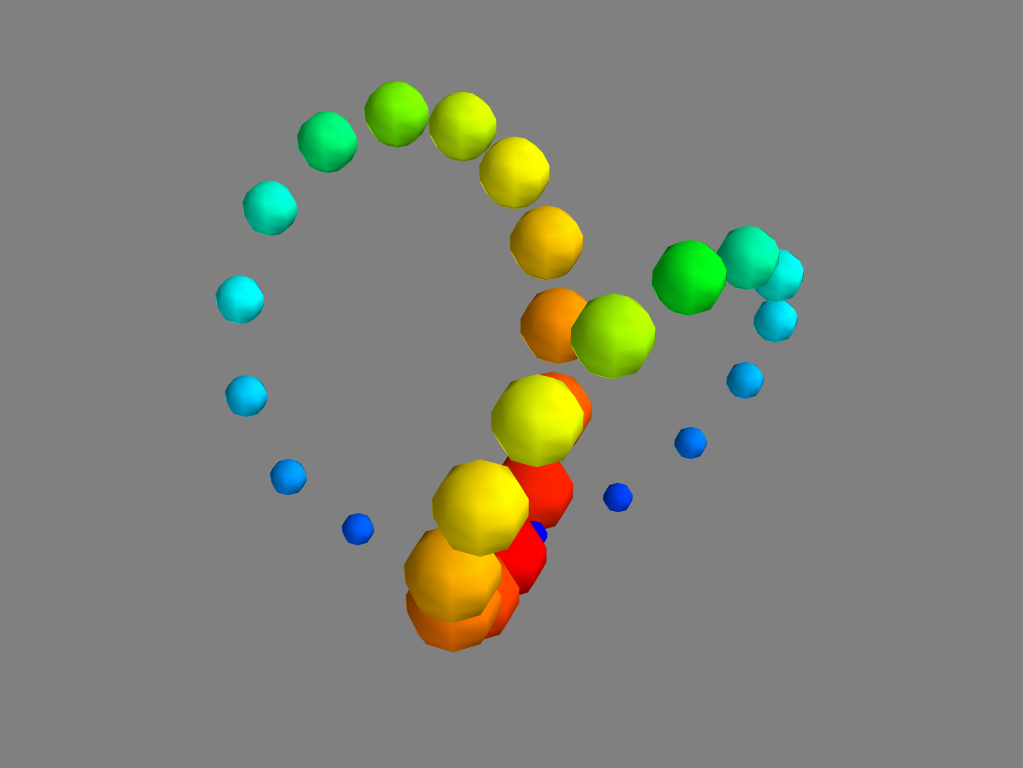
\includegraphics[width=\linewidth]{points3d.png}
    \caption{A 3-D scatter plot generated by \li{mlab.points3d()}.}
    \label{fig:points3d}
\end{subfigure}
\end{figure}

\subsection*{Points} % --------------------------------------------------------

The function \li{mlab.points3d()} is the 3-D Mayavi equivalent for Matplotlib's \li{plt.scatter()}.
Each point is plotted, but not connected with lines.
In the code below, the optional input array \li{s} defines a scalar for each point that modifies the color and size of the point.
The output is in Figure \ref{fig:points3d}.

\begin{lstlisting}
>>> t = np.linspace(0, 4*np.pi, 30)
>>> x = np.sin(2*t)
>>> y = np.cos(t)
>>> z = np.cos(2*t)
>>> s = 2 + np.sin(t)

# Adjust the keyword argument 'scale_factor' so all points are visible.
>>> mlab.points3d(x, y, z, s, scale_factor=.15)
>>> mlab.show()
\end{lstlisting}

\subsection*{Surfaces} % ------------------------------------------------------

The function \li{mlab.surf()} renders a 3-D surface.
Because the surface is over a 2-D domain, we create a coordinate grid with \li{np.mgrid()} (similar to \li{np.meshgrid()}).
This function uses the slicing syntax \li{[start:stop:step]}, similar to \li{range()} and \li{np.arange()}, but is accessed with brackets instead of parentheses.

The following code produces the hyperbolic paraboloid $f(x,y) = \frac{x^2}{4} - \frac{y^2}{4}$ over the domain $[-4,4]\times[-4,4]$.
The result is displayed in Figure \ref{fig:surf_example}.

\begin{lstlisting}
>>> X, Y = np.mgrid[-4:4:.025, -4:4:.025]
>>> Z = (X**2)/4. - (Y**2)/4.
>>> mlab.surf(X, Y, Z, colormap='RdYlGn')
>>> mlab.show()
\end{lstlisting}

\begin{figure}
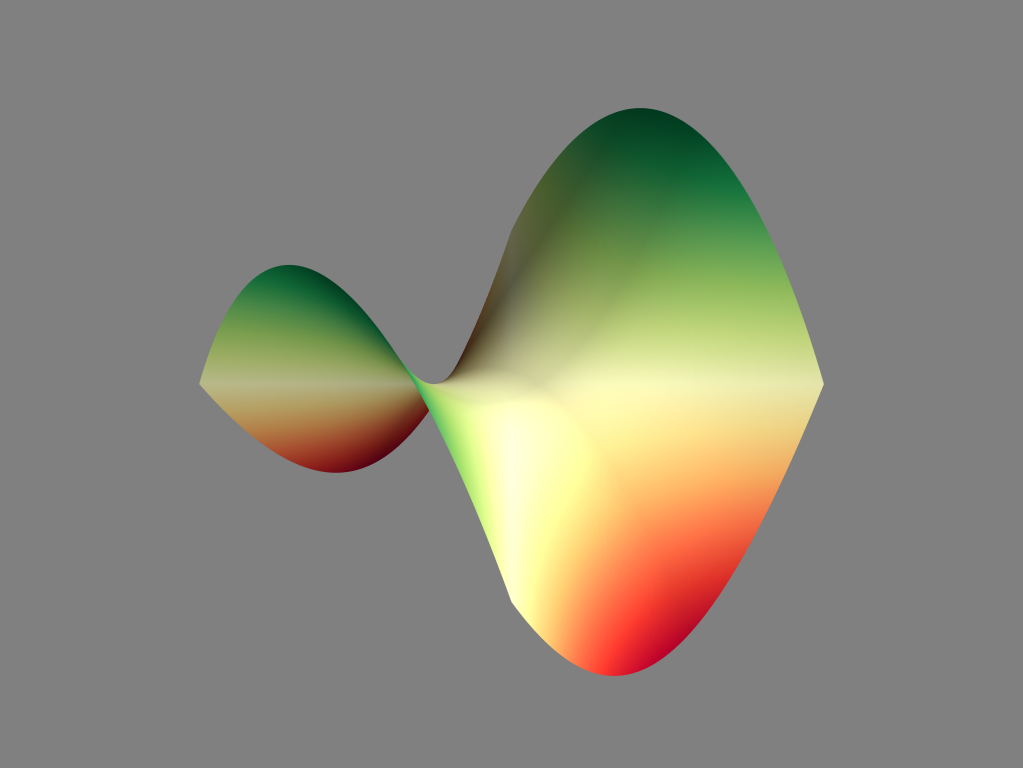
\includegraphics[width=.7\textwidth]{mesh_example.png}
\caption{Sample output of \li{mlab.surf()}.}
\label{fig:surf_example}
\end{figure}

Like Matplotlib, Mayavi supports various color schemes, either as a solid color or with a varying colormap.
For example, the plot in Figure \ref{fig:surf_example} uses the colormap \li{'RdYlGn'}.
For a list of all colormaps in Mayavi, see \url{http://docs.enthought.com/mayavi/mayavi/mlab_changing_object_looks.html}.

% TODO: More exercises with Mayavi!!! Don't have to be too hard either...
\begin{problem}
Plot the function $z = \frac{1}{10}\sin(10(x^2+y^2))$ on $[-1,1] \times [-1,1]$ using Mayavi.
\end{problem}

% TODO: this problem is copied from https://github.com/enthought/mayavi/blob/master/examples/mayavi/mlab/canyon.py.
% We need to find a different problem.
\begin{comment}
\begin{problem}
\label{prob:grand_canyon}
Provided Grand Canyon topological radar data from NASA, do the following.

\begin{itemize}
\item Reshape the data to be 3601x3601.
\item Cast the data type as \li{float32}.
\item Slice the data, taking the first 1000 rows and columns 900-1900.
\item There is some missing data, so set the minimum of your data equal to the minimum of the the positive data points.
\item Preset the figure using the following commands: \li{mlab.figure(size=(400,320)}, \li{bgcolor = (.16, .28, .46))}
\item Now plot with \li{mlab.surf}, using the colormap \li{gist_earth}, with a \li{warp_scale=.2}, \li{vmin=1200}, and \li{vmax=1610}.
\item Take a smaller view of the canyon using \li{mlab.view(-5.9, 83, 570, [5.3, 20, 238])}.
\end{itemize}

This should produce Figure \ref{fig:GrandCanyon}

\begin{figure}[H]
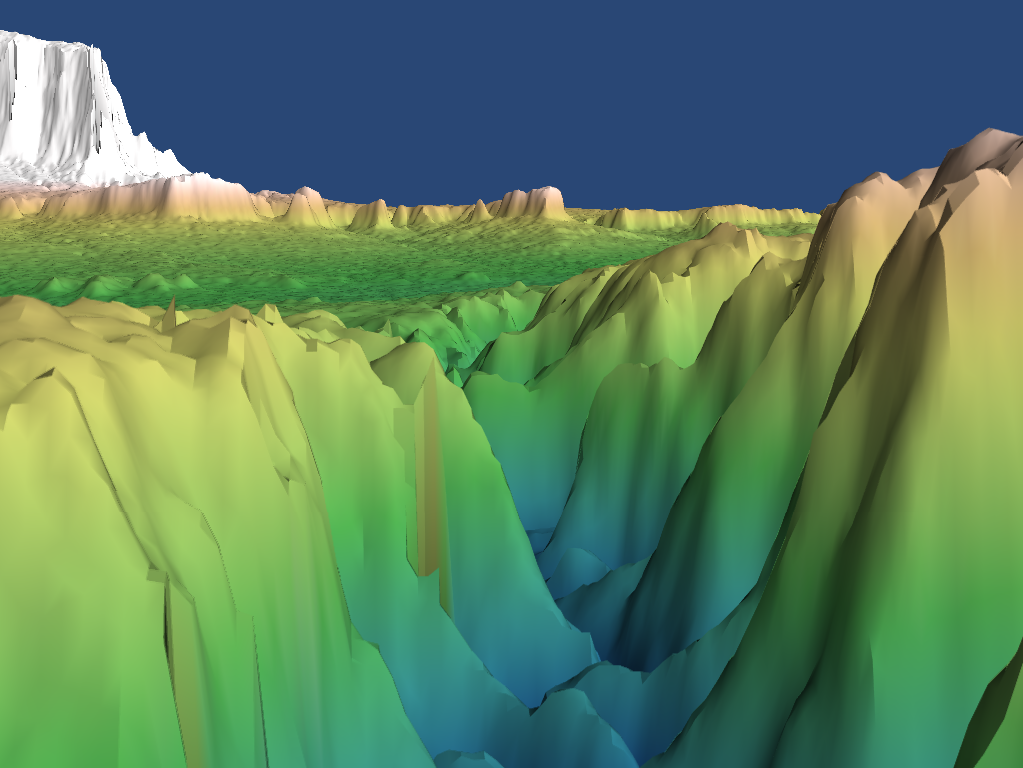
\includegraphics[width=.7\textwidth]{GrandCanyon.png}
\caption{Correct output for Problem \ref{prob:grand_canyon}.}
\label{fig:GrandCanyon}
\end{figure}

\end{problem}
\end{comment}

\newpage

\section*{Additional Material} % ==============================================

\subsection*{3-D Plotting with Matplotlib} % ----------------------------------

Matplotlib can also be used for 3D plotting, though it is much slower and not as visually appealing as Mayavi plots.
The following code produces Figure \ref{fig:surface}.

\begin{lstlisting}
# Create the domain and calculate the range.
>>> x = np.linspace(-np.pi, np.pi, n)
>>> y = np.copy(x)
>>> X, Y = np.meshgrid(x, y)
>>> Z = np.sin(X)*np.sin(Y)

# Draw the corresponding 3-D plot.
>>> from mpl_toolkits.mplot3d import Axes3D
>>> fig = plt.figure()
>>> ax = fig.gca(projection='3d')
>>> ax.plot_surface(X, Y, Z)
>>> plt.show()
\end{lstlisting}

\begin{comment}
\begin{problem}
Plot the function $\frac{\cos\left(\sqrt{x^2 + y^2}\right)}{\frac{x^2 + y^2}{10} + 1}$ on $[-10, 10] \times [-10, 10]$.
\end{problem}
\end{comment}

\subsection*{Interactive Plots}

Matplotlib plots can be made interactive by adding \emph{widgets}.
Consider the following example, TAKEN FROM THE MATPLOTLIB DOCS BASICALLY AHHH

\begin{lstlisting} 
>>> from matplotlib import widgets as wg 

>>> ax = plt.subplot(111)
>>> plt.subplots_adjust(bottom=.25)         # Make some space for a slider bar.
>>> t = np.arange(0., 1., .001)     
>>> a0 = 5. 
>>> f0 = 3. 
>>> s = a0 * np.sin(2 * np.pi * f0 * t) 
>>> l = plt.plot(t, s)[0]
>>> plt.axis([0, 1, -10, 10]) 
>>> axfreq = plt.axes([.25, .05, .65, .03]) 
>>> axamp = plt.axes([.25, .1, .65, .03]) 

# Make some slider bars.
>>> sfreq = wg.Slider(axfreq, 'Freq', .1, 30., valinit=f0) 
>>> samp = wg.Slider(axamp, 'Amp', .1, 10., valinit=a0) 
>>> def update(val):                        # Function for updating the plot.
...     amp = samp.val                          # Read from one slider.
...     freq = sfreq.val                        # Read from the other slider.
...     l.set_ydata(amp * np.sin(2 * np.pi * freq * t)) 
...     plt.draw()                              # Refresh the plot.
>>> sfreq.on_changed(update)                # Connect the sliders to update().
>>> samp.on_changed(update)
>>> plt.show() 
\end{lstlisting}

\begin{figure}[H]
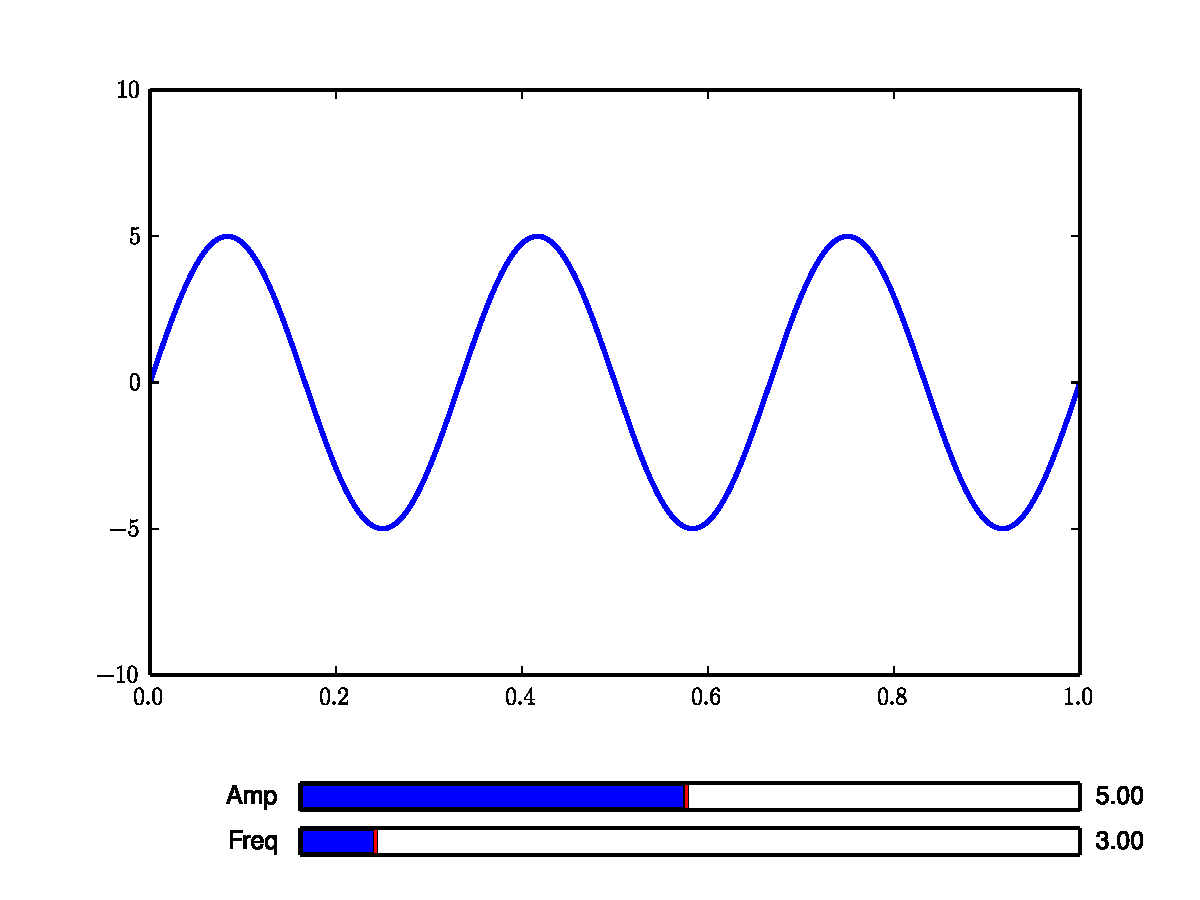
\includegraphics[width=.7\textwidth]{interact.pdf}
\caption{A snapshot of an interactive plot made using Matplotlib.}
\label{mpl:interact} \end{figure}

% \begin{problem} Modify the code above to add a third slider to
% manipulate the phase of the wave shown. Have it range from 0 to $2\pi$
% and set the default value to zero. \end{problem}

\subsection*{Animations} % ----------------------------------------------------

Stuff from Volume 4.

% =============================================================================
% =============================================================================
% Stuff to move ===============================================================
% =============================================================================
% =============================================================================

\begin{comment}
\begin{info} % IPython Notebook inline plotting (move to another lab!)
If you are executing these Matplotlib commands in an IPython shell, executing the \li{plt.show} method will open a new window with the plot. If you are using IPython Notebook, you have the option to display the plots within your notebook. You may opt into this feature by running \li{\%matplotlib inline} or \li{\%matplotlib notebook} in your IPython Notebook. The \li{inline} option shows the plot, whereas the \li{notebook} option shows the plot and provides controls to interact with the plot. Additionally, when using this option, the plot is displayed after running the \li{plt.plot} command; the \li{plt.show} command is not necessary. 
\end{info}
\end{comment}


\begin{comment} % This will be covered in the Complex labs.
\begin{problem} Use \li{plt.pcolormesh()} to plot the absolute value of the function $x^3 +2x^2 -x +3$ on the complex plane with 0 $\leq$ \li{x} $\leq$ 2 and 0 $\leq$ \li{y} $\leq$ 2.
\emph{Helpful Hint}: First create your domain arrays, then convert these to a single array of complex variables to evaluate the function.

The plot should look like Figure \ref{fig:pcolormesh}.

\begin{figure}[H] % Complex colorplot
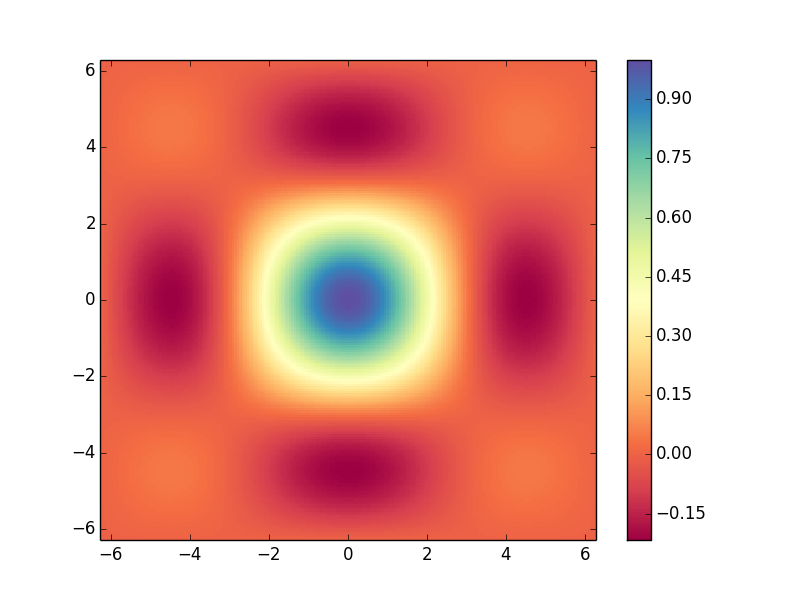
\includegraphics[width=\textwidth]{pcolor2.png}
\caption{Another example of a colorplot.}
\label{fig:pcolormesh}
\end{figure}
\end{problem}
\end{comment}
